\documentclass[12pt,a4paper,]{book}
\def\ifdoblecara{} %% set to true
\def\ifprincipal{} %% set to true
\let\ifprincipal\undefined %% set to false
\def\ifcitapandoc{} %% set to true
\let\ifcitapandoc\undefined %% set to false
\usepackage{lmodern}
% sin fontmathfamily
\usepackage{amssymb,amsmath}
\usepackage{ifxetex,ifluatex}
%\usepackage{fixltx2e} % provides \textsubscript %PLLC
\ifnum 0\ifxetex 1\fi\ifluatex 1\fi=0 % if pdftex
  \usepackage[T1]{fontenc}
  \usepackage[utf8]{inputenc}
\else % if luatex or xelatex
  \ifxetex
    \usepackage{mathspec}
  \else
    \usepackage{fontspec}
  \fi
  \defaultfontfeatures{Ligatures=TeX,Scale=MatchLowercase}
\fi
% use upquote if available, for straight quotes in verbatim environments
\IfFileExists{upquote.sty}{\usepackage{upquote}}{}
% use microtype if available
\IfFileExists{microtype.sty}{%
\usepackage{microtype}
\UseMicrotypeSet[protrusion]{basicmath} % disable protrusion for tt fonts
}{}
\usepackage[margin = 2.5cm]{geometry}
\usepackage{hyperref}
\hypersetup{unicode=true,
            pdfauthor={Nombre Completo Autor},
              pdfborder={0 0 0},
              breaklinks=true}
\urlstyle{same}  % don't use monospace font for urls
%
\usepackage[usenames,dvipsnames]{xcolor}  %new PLLC
\usepackage{color}
\usepackage{fancyvrb}
\newcommand{\VerbBar}{|}
\newcommand{\VERB}{\Verb[commandchars=\\\{\}]}
\DefineVerbatimEnvironment{Highlighting}{Verbatim}{commandchars=\\\{\}}
% Add ',fontsize=\small' for more characters per line
\usepackage{framed}
\definecolor{shadecolor}{RGB}{248,248,248}
\newenvironment{Shaded}{\begin{snugshade}}{\end{snugshade}}
\newcommand{\AlertTok}[1]{\textcolor[rgb]{0.94,0.16,0.16}{#1}}
\newcommand{\AnnotationTok}[1]{\textcolor[rgb]{0.56,0.35,0.01}{\textbf{\textit{#1}}}}
\newcommand{\AttributeTok}[1]{\textcolor[rgb]{0.13,0.29,0.53}{#1}}
\newcommand{\BaseNTok}[1]{\textcolor[rgb]{0.00,0.00,0.81}{#1}}
\newcommand{\BuiltInTok}[1]{#1}
\newcommand{\CharTok}[1]{\textcolor[rgb]{0.31,0.60,0.02}{#1}}
\newcommand{\CommentTok}[1]{\textcolor[rgb]{0.56,0.35,0.01}{\textit{#1}}}
\newcommand{\CommentVarTok}[1]{\textcolor[rgb]{0.56,0.35,0.01}{\textbf{\textit{#1}}}}
\newcommand{\ConstantTok}[1]{\textcolor[rgb]{0.56,0.35,0.01}{#1}}
\newcommand{\ControlFlowTok}[1]{\textcolor[rgb]{0.13,0.29,0.53}{\textbf{#1}}}
\newcommand{\DataTypeTok}[1]{\textcolor[rgb]{0.13,0.29,0.53}{#1}}
\newcommand{\DecValTok}[1]{\textcolor[rgb]{0.00,0.00,0.81}{#1}}
\newcommand{\DocumentationTok}[1]{\textcolor[rgb]{0.56,0.35,0.01}{\textbf{\textit{#1}}}}
\newcommand{\ErrorTok}[1]{\textcolor[rgb]{0.64,0.00,0.00}{\textbf{#1}}}
\newcommand{\ExtensionTok}[1]{#1}
\newcommand{\FloatTok}[1]{\textcolor[rgb]{0.00,0.00,0.81}{#1}}
\newcommand{\FunctionTok}[1]{\textcolor[rgb]{0.13,0.29,0.53}{\textbf{#1}}}
\newcommand{\ImportTok}[1]{#1}
\newcommand{\InformationTok}[1]{\textcolor[rgb]{0.56,0.35,0.01}{\textbf{\textit{#1}}}}
\newcommand{\KeywordTok}[1]{\textcolor[rgb]{0.13,0.29,0.53}{\textbf{#1}}}
\newcommand{\NormalTok}[1]{#1}
\newcommand{\OperatorTok}[1]{\textcolor[rgb]{0.81,0.36,0.00}{\textbf{#1}}}
\newcommand{\OtherTok}[1]{\textcolor[rgb]{0.56,0.35,0.01}{#1}}
\newcommand{\PreprocessorTok}[1]{\textcolor[rgb]{0.56,0.35,0.01}{\textit{#1}}}
\newcommand{\RegionMarkerTok}[1]{#1}
\newcommand{\SpecialCharTok}[1]{\textcolor[rgb]{0.81,0.36,0.00}{\textbf{#1}}}
\newcommand{\SpecialStringTok}[1]{\textcolor[rgb]{0.31,0.60,0.02}{#1}}
\newcommand{\StringTok}[1]{\textcolor[rgb]{0.31,0.60,0.02}{#1}}
\newcommand{\VariableTok}[1]{\textcolor[rgb]{0.00,0.00,0.00}{#1}}
\newcommand{\VerbatimStringTok}[1]{\textcolor[rgb]{0.31,0.60,0.02}{#1}}
\newcommand{\WarningTok}[1]{\textcolor[rgb]{0.56,0.35,0.01}{\textbf{\textit{#1}}}}

% PLLC modifica-ini
% PLLC modifica-fin

\IfFileExists{parskip.sty}{%
\usepackage{parskip}
}{% else
\setlength{\parindent}{0pt}
\setlength{\parskip}{6pt plus 2pt minus 1pt}
}
\setlength{\emergencystretch}{3em}  % prevent overfull lines
\providecommand{\tightlist}{%
  \setlength{\itemsep}{0pt}\setlength{\parskip}{0pt}}
\setcounter{secnumdepth}{5}
% Redefines (sub)paragraphs to behave more like sections
\ifx\paragraph\undefined\else
\let\oldparagraph\paragraph
\renewcommand{\paragraph}[1]{\oldparagraph{#1}\mbox{}}
\fi
\ifx\subparagraph\undefined\else
\let\oldsubparagraph\subparagraph
\renewcommand{\subparagraph}[1]{\oldsubparagraph{#1}\mbox{}}
\fi

%%% Use protect on footnotes to avoid problems with footnotes in titles
\let\rmarkdownfootnote\footnote%
\def\footnote{\protect\rmarkdownfootnote}


  \title{}
    \author{Nombre Completo Autor}
      \date{18/11/2021}


%%%%%%% inicio: latex_preambulo.tex PLLC


%% UTILIZA CODIFICACIÓN UTF-8
%% MODIFICARLO CONVENIENTEMENTE PARA USARLO CON OTRAS CODIFICACIONES


%\usepackage[spanish,es-nodecimaldot,es-noshorthands]{babel}
\usepackage[spanish,es-nodecimaldot,es-noshorthands,es-tabla]{babel}
% Ver: es-tabla (en: https://osl.ugr.es/CTAN/macros/latex/contrib/babel-contrib/spanish/spanish.pdf)
% es-tabla (en: https://tex.stackexchange.com/questions/80443/change-the-word-table-in-table-captions)
\usepackage[spanish, plain, datebegin,sortcompress,nocomment,
noabstract]{flexbib}
 
\usepackage{float}
\usepackage{placeins}
\usepackage{fancyhdr}
% Solucion: ! LaTeX Error: Command \counterwithout already defined.
% https://tex.stackexchange.com/questions/425600/latex-error-command-counterwithout-already-defined
\let\counterwithout\relax
\let\counterwithin\relax
\usepackage{chngcntr}
%\usepackage{microtype}  %antes en template PLLC
\usepackage[utf8]{inputenc}
\usepackage[T1]{fontenc} % Usa codificación 8-bit que tiene 256 glyphs

%\usepackage[dvipsnames]{xcolor}
%\usepackage[usenames,dvipsnames]{xcolor}  %new
\usepackage{pdfpages}
%\usepackage{natbib}




% Para portada: latex_paginatitulo_mod_ST02.tex (inicio)
\usepackage{tikz}
\usepackage{epigraph}
\renewcommand\epigraphflush{flushright}
\renewcommand\epigraphsize{\normalsize}
\setlength\epigraphwidth{0.7\textwidth}

\definecolor{titlepagecolor}{cmyk}{1,.60,0,.40}

%\DeclareFixedFont{\titlefont}{T1}{ppl}{b}{it}{0.5in}

% \makeatletter
% \def\printauthor{%
%     {\large \@author}}
% \makeatother
% \author{%
%     Author 1 name \\
%     Department name \\
%     \texttt{email1@example.com}\vspace{20pt} \\
%     Author 2 name \\
%     Department name \\
%     \texttt{email2@example.com}
%     }

% The following code is borrowed from: https://tex.stackexchange.com/a/86310/10898

\newcommand\titlepagedecoration{%
\begin{tikzpicture}[remember picture,overlay,shorten >= -10pt]

\coordinate (aux1) at ([yshift=-15pt]current page.north east);
\coordinate (aux2) at ([yshift=-410pt]current page.north east);
\coordinate (aux3) at ([xshift=-4.5cm]current page.north east);
\coordinate (aux4) at ([yshift=-150pt]current page.north east);

\begin{scope}[titlepagecolor!40,line width=12pt,rounded corners=12pt]
\draw
  (aux1) -- coordinate (a)
  ++(225:5) --
  ++(-45:5.1) coordinate (b);
\draw[shorten <= -10pt]
  (aux3) --
  (a) --
  (aux1);
\draw[opacity=0.6,titlepagecolor,shorten <= -10pt]
  (b) --
  ++(225:2.2) --
  ++(-45:2.2);
\end{scope}
\draw[titlepagecolor,line width=8pt,rounded corners=8pt,shorten <= -10pt]
  (aux4) --
  ++(225:0.8) --
  ++(-45:0.8);
\begin{scope}[titlepagecolor!70,line width=6pt,rounded corners=8pt]
\draw[shorten <= -10pt]
  (aux2) --
  ++(225:3) coordinate[pos=0.45] (c) --
  ++(-45:3.1);
\draw
  (aux2) --
  (c) --
  ++(135:2.5) --
  ++(45:2.5) --
  ++(-45:2.5) coordinate[pos=0.3] (d);   
\draw 
  (d) -- +(45:1);
\end{scope}
\end{tikzpicture}%
}

% Para portada: latex_paginatitulo_mod_ST02.tex (fin)

% Para portada: latex_paginatitulo_mod_OV01.tex (inicio)
\usepackage{cpimod}
% Para portada: latex_paginatitulo_mod_OV01.tex (fin)

% Para portada: latex_paginatitulo_mod_OV03.tex (inicio)
\usepackage{KTHEEtitlepage}
% Para portada: latex_paginatitulo_mod_OV03.tex (fin)

\renewcommand{\contentsname}{Índice}
\renewcommand{\listfigurename}{Índice de figuras}
\renewcommand{\listtablename}{Índice de tablas}
\newcommand{\bcols}{}
\newcommand{\ecols}{}
\newcommand{\bcol}[1]{\begin{minipage}{#1\linewidth}}
\newcommand{\ecol}{\end{minipage}}
\newcommand{\balertblock}[1]{\begin{alertblock}{#1}}
\newcommand{\ealertblock}{\end{alertblock}}
\newcommand{\bitemize}{\begin{itemize}}
\newcommand{\eitemize}{\end{itemize}}
\newcommand{\benumerate}{\begin{enumerate}}
\newcommand{\eenumerate}{\end{enumerate}}
\newcommand{\saltopagina}{\newpage}
\newcommand{\bcenter}{\begin{center}}
\newcommand{\ecenter}{\end{center}}
\newcommand{\beproof}{\begin{proof}} %new
\newcommand{\eeproof}{\end{proof}} %new
%De: https://texblog.org/2007/11/07/headerfooter-in-latex-with-fancyhdr/
% \fancyhead
% E: Even page
% O: Odd page
% L: Left field
% C: Center field
% R: Right field
% H: Header
% F: Footer
%\fancyhead[CO,CE]{Resultados}

%OPCION 1
% \fancyhead[LE,RO]{\slshape \rightmark}
% \fancyhead[LO,RE]{\slshape \leftmark}
% \fancyfoot[C]{\thepage}
% \renewcommand{\headrulewidth}{0.4pt}
% \renewcommand{\footrulewidth}{0pt}

%OPCION 2
% \fancyhead[LE,RO]{\slshape \rightmark}
% \fancyfoot[LO,RE]{\slshape \leftmark}
% \fancyfoot[LE,RO]{\thepage}
% \renewcommand{\headrulewidth}{0.4pt}
% \renewcommand{\footrulewidth}{0.4pt}
%%%%%%%%%%
\usepackage{calc,amsfonts}
% Elimina la cabecera de páginas impares vacías al finalizar los capítulos
\usepackage{emptypage}
\makeatletter

%\definecolor{ocre}{RGB}{25,25,243} % Define el color azul (naranja) usado para resaltar algunas salidas
\definecolor{ocre}{RGB}{0,0,0} % Define el color a negro (aparece en los teoremas

%\usepackage{calc} 


%era if(csl-refs) con dolares
% metodobib: true


\usepackage{lipsum}

%\usepackage{tikz} % Requerido para dibujar formas personalizadas

%\usepackage{amsmath,amsthm,amssymb,amsfonts}
\usepackage{amsthm}


% Boxed/framed environments
\newtheoremstyle{ocrenumbox}% % Theorem style name
{0pt}% Space above
{0pt}% Space below
{\normalfont}% % Body font
{}% Indent amount
{\small\bf\sffamily\color{ocre}}% % Theorem head font
{\;}% Punctuation after theorem head
{0.25em}% Space after theorem head
{\small\sffamily\color{ocre}\thmname{#1}\nobreakspace\thmnumber{\@ifnotempty{#1}{}\@upn{#2}}% Theorem text (e.g. Theorem 2.1)
\thmnote{\nobreakspace\the\thm@notefont\sffamily\bfseries\color{black}---\nobreakspace#3.}} % Optional theorem note
\renewcommand{\qedsymbol}{$\blacksquare$}% Optional qed square

\newtheoremstyle{blacknumex}% Theorem style name
{5pt}% Space above
{5pt}% Space below
{\normalfont}% Body font
{} % Indent amount
{\small\bf\sffamily}% Theorem head font
{\;}% Punctuation after theorem head
{0.25em}% Space after theorem head
{\small\sffamily{\tiny\ensuremath{\blacksquare}}\nobreakspace\thmname{#1}\nobreakspace\thmnumber{\@ifnotempty{#1}{}\@upn{#2}}% Theorem text (e.g. Theorem 2.1)
\thmnote{\nobreakspace\the\thm@notefont\sffamily\bfseries---\nobreakspace#3.}}% Optional theorem note

\newtheoremstyle{blacknumbox} % Theorem style name
{0pt}% Space above
{0pt}% Space below
{\normalfont}% Body font
{}% Indent amount
{\small\bf\sffamily}% Theorem head font
{\;}% Punctuation after theorem head
{0.25em}% Space after theorem head
{\small\sffamily\thmname{#1}\nobreakspace\thmnumber{\@ifnotempty{#1}{}\@upn{#2}}% Theorem text (e.g. Theorem 2.1)
\thmnote{\nobreakspace\the\thm@notefont\sffamily\bfseries---\nobreakspace#3.}}% Optional theorem note

% Non-boxed/non-framed environments
\newtheoremstyle{ocrenum}% % Theorem style name
{5pt}% Space above
{5pt}% Space below
{\normalfont}% % Body font
{}% Indent amount
{\small\bf\sffamily\color{ocre}}% % Theorem head font
{\;}% Punctuation after theorem head
{0.25em}% Space after theorem head
{\small\sffamily\color{ocre}\thmname{#1}\nobreakspace\thmnumber{\@ifnotempty{#1}{}\@upn{#2}}% Theorem text (e.g. Theorem 2.1)
\thmnote{\nobreakspace\the\thm@notefont\sffamily\bfseries\color{black}---\nobreakspace#3.}} % Optional theorem note
\renewcommand{\qedsymbol}{$\blacksquare$}% Optional qed square
\makeatother



% Define el estilo texto theorem para cada tipo definido anteriormente
\newcounter{dummy} 
\numberwithin{dummy}{section}
\theoremstyle{ocrenumbox}
\newtheorem{theoremeT}[dummy]{Teorema}  % (Pedro: Theorem)
\newtheorem{problem}{Problema}[chapter]  % (Pedro: Problem)
\newtheorem{exerciseT}{Ejercicio}[chapter] % (Pedro: Exercise)
\theoremstyle{blacknumex}
\newtheorem{exampleT}{Ejemplo}[chapter] % (Pedro: Example)
\theoremstyle{blacknumbox}
\newtheorem{vocabulary}{Vocabulario}[chapter]  % (Pedro: Vocabulary)
\newtheorem{definitionT}{Definición}[section]  % (Pedro: Definition)
\newtheorem{corollaryT}[dummy]{Corolario}  % (Pedro: Corollary)
\theoremstyle{ocrenum}
\newtheorem{proposition}[dummy]{Proposición} % (Pedro: Proposition)


\usepackage[framemethod=default]{mdframed}



\newcommand{\intoo}[2]{\mathopen{]}#1\,;#2\mathclose{[}}
\newcommand{\ud}{\mathop{\mathrm{{}d}}\mathopen{}}
\newcommand{\intff}[2]{\mathopen{[}#1\,;#2\mathclose{]}}
\newtheorem{notation}{Notation}[chapter]


\mdfdefinestyle{exampledefault}{%
rightline=true,innerleftmargin=10,innerrightmargin=10,
frametitlerule=true,frametitlerulecolor=green,
frametitlebackgroundcolor=yellow,
frametitlerulewidth=2pt}


% Theorem box
\newmdenv[skipabove=7pt,
skipbelow=7pt,
backgroundcolor=black!5,
linecolor=ocre,
innerleftmargin=5pt,
innerrightmargin=5pt,
innertopmargin=10pt,%5pt
leftmargin=0cm,
rightmargin=0cm,
innerbottommargin=5pt]{tBox}

% Exercise box	  
\newmdenv[skipabove=7pt,
skipbelow=7pt,
rightline=false,
leftline=true,
topline=false,
bottomline=false,
backgroundcolor=ocre!10,
linecolor=ocre,
innerleftmargin=5pt,
innerrightmargin=5pt,
innertopmargin=10pt,%5pt
innerbottommargin=5pt,
leftmargin=0cm,
rightmargin=0cm,
linewidth=4pt]{eBox}	

% Definition box
\newmdenv[skipabove=7pt,
skipbelow=7pt,
rightline=false,
leftline=true,
topline=false,
bottomline=false,
linecolor=ocre,
innerleftmargin=5pt,
innerrightmargin=5pt,
innertopmargin=10pt,%0pt
leftmargin=0cm,
rightmargin=0cm,
linewidth=4pt,
innerbottommargin=0pt]{dBox}	

% Corollary box
\newmdenv[skipabove=7pt,
skipbelow=7pt,
rightline=false,
leftline=true,
topline=false,
bottomline=false,
linecolor=gray,
backgroundcolor=black!5,
innerleftmargin=5pt,
innerrightmargin=5pt,
innertopmargin=10pt,%5pt
leftmargin=0cm,
rightmargin=0cm,
linewidth=4pt,
innerbottommargin=5pt]{cBox}

% Crea un entorno para cada tipo de theorem y le asigna un estilo 
% con ayuda de las cajas coloreadas anteriores
\newenvironment{theorem}{\begin{tBox}\begin{theoremeT}}{\end{theoremeT}\end{tBox}}
\newenvironment{exercise}{\begin{eBox}\begin{exerciseT}}{\hfill{\color{ocre}\tiny\ensuremath{\blacksquare}}\end{exerciseT}\end{eBox}}				  
\newenvironment{definition}{\begin{dBox}\begin{definitionT}}{\end{definitionT}\end{dBox}}	
\newenvironment{example}{\begin{exampleT}}{\hfill{\tiny\ensuremath{\blacksquare}}\end{exampleT}}		
\newenvironment{corollary}{\begin{cBox}\begin{corollaryT}}{\end{corollaryT}\end{cBox}}	

%	ENVIRONMENT remark
\newenvironment{remark}{\par\vspace{10pt}\small 
% Espacio blanco vertical sobre la nota y tamaño de fuente menor
\begin{list}{}{
\leftmargin=35pt % Indentación sobre la izquierda
\rightmargin=25pt}\item\ignorespaces % Indentación sobre la derecha
\makebox[-2.5pt]{\begin{tikzpicture}[overlay]
\node[draw=ocre!60,line width=1pt,circle,fill=ocre!25,font=\sffamily\bfseries,inner sep=2pt,outer sep=0pt] at (-15pt,0pt){\textcolor{ocre}{N}}; \end{tikzpicture}} % R naranja en un círculo (Pedro)
\advance\baselineskip -1pt}{\end{list}\vskip5pt} 
% Espaciado de línea más estrecho y espacio en blanco después del comentario


\newenvironment{solutionExe}{\par\vspace{10pt}\small 
\begin{list}{}{
\leftmargin=35pt 
\rightmargin=25pt}\item\ignorespaces 
\makebox[-2.5pt]{\begin{tikzpicture}[overlay]
\node[draw=ocre!60,line width=1pt,circle,fill=ocre!25,font=\sffamily\bfseries,inner sep=2pt,outer sep=0pt] at (-15pt,0pt){\textcolor{ocre}{S}}; \end{tikzpicture}} 
\advance\baselineskip -1pt}{\end{list}\vskip5pt} 

\newenvironment{solutionExa}{\par\vspace{10pt}\small 
\begin{list}{}{
\leftmargin=35pt 
\rightmargin=25pt}\item\ignorespaces 
\makebox[-2.5pt]{\begin{tikzpicture}[overlay]
\node[draw=ocre!60,line width=1pt,circle,fill=ocre!55,font=\sffamily\bfseries,inner sep=2pt,outer sep=0pt] at (-15pt,0pt){\textcolor{ocre}{S}}; \end{tikzpicture}} 
\advance\baselineskip -1pt}{\end{list}\vskip5pt} 

\usepackage{tcolorbox}

\usetikzlibrary{trees}

\theoremstyle{ocrenum}
\newtheorem{solutionT}[dummy]{Solución}  % (Pedro: Corollary)
\newenvironment{solution}{\begin{cBox}\begin{solutionT}}{\end{solutionT}\end{cBox}}	


\newcommand{\tcolorboxsolucion}[2]{%
\begin{tcolorbox}[colback=green!5!white,colframe=green!75!black,title=#1] 
 #2
 %\tcblower  % pone una línea discontinua
\end{tcolorbox}
}% final definición comando

\newtcbox{\mybox}[1][green]{on line,
arc=0pt,outer arc=0pt,colback=#1!10!white,colframe=#1!50!black, boxsep=0pt,left=1pt,right=1pt,top=2pt,bottom=2pt, boxrule=0pt,bottomrule=1pt,toprule=1pt}



\mdfdefinestyle{exampledefault}{%
rightline=true,innerleftmargin=10,innerrightmargin=10,
frametitlerule=true,frametitlerulecolor=green,
frametitlebackgroundcolor=yellow,
frametitlerulewidth=2pt}





\newcommand{\betheorem}{\begin{theorem}}
\newcommand{\eetheorem}{\end{theorem}}
\newcommand{\bedefinition}{\begin{definition}}
\newcommand{\eedefinition}{\end{definition}}

\newcommand{\beremark}{\begin{remark}}
\newcommand{\eeremark}{\end{remark}}
\newcommand{\beexercise}{\begin{exercise}}
\newcommand{\eeexercise}{\end{exercise}}
\newcommand{\beexample}{\begin{example}}
\newcommand{\eeexample}{\end{example}}
\newcommand{\becorollary}{\begin{corollary}}
\newcommand{\eecorollary}{\end{corollary}}


\newcommand{\besolutionExe}{\begin{solutionExe}}
\newcommand{\eesolutionExe}{\end{solutionExe}}
\newcommand{\besolutionExa}{\begin{solutionExa}}
\newcommand{\eesolutionExa}{\end{solutionExa}}


%%%%%%%%


% Caja Salida Markdown
\newmdenv[skipabove=7pt,
skipbelow=7pt,
rightline=false,
leftline=true,
topline=false,
bottomline=false,
backgroundcolor=GreenYellow!10,
linecolor=GreenYellow!80,
innerleftmargin=5pt,
innerrightmargin=5pt,
innertopmargin=10pt,%5pt
innerbottommargin=5pt,
leftmargin=0cm,
rightmargin=0cm,
linewidth=4pt]{mBox}	

%% RMarkdown
\newenvironment{markdownsal}{\begin{mBox}}{\end{mBox}}	

\newcommand{\bmarkdownsal}{\begin{markdownsal}}
\newcommand{\emarkdownsal}{\end{markdownsal}}


\usepackage{array}
\usepackage{multirow}
\usepackage{wrapfig}
\usepackage{colortbl}
\usepackage{pdflscape}
\usepackage{tabu}
\usepackage{threeparttable}
\usepackage{subfig} %new
%\usepackage{booktabs,dcolumn,rotating,thumbpdf,longtable}
\usepackage{dcolumn,rotating}  %new
\usepackage[graphicx]{realboxes} %new de: https://stackoverflow.com/questions/51633434/prevent-pagebreak-in-kableextra-landscape-table

%define el interlineado vertical
%\renewcommand{\baselinestretch}{1.5}

%define etiqueta para las Tablas o Cuadros
%\renewcommand\spanishtablename{Tabla}

%%\bibliographystyle{plain} %new no necesario


%%%%%%%%%%%% PARA USO CON biblatex
% \DefineBibliographyStrings{english}{%
%   backrefpage = {ver pag.\adddot},%
%   backrefpages = {ver pags.\adddot}%
% }

% \DefineBibliographyStrings{spanish}{%
%   backrefpage = {ver pag.\adddot},%
%   backrefpages = {ver pags.\adddot}%
% }
% 
% \DeclareFieldFormat{pagerefformat}{\mkbibparens{{\color{red}\mkbibemph{#1}}}}
% \renewbibmacro*{pageref}{%
%   \iflistundef{pageref}
%     {}
%     {\printtext[pagerefformat]{%
%        \ifnumgreater{\value{pageref}}{1}
%          {\bibstring{backrefpages}\ppspace}
%          {\bibstring{backrefpage}\ppspace}%
%        \printlist[pageref][-\value{listtotal}]{pageref}}}}
% 
%%% de kableExtra
\usepackage{booktabs}
\usepackage{longtable}
%\usepackage{array}
%\usepackage{multirow}
%\usepackage{wrapfig}
%\usepackage{float}
%\usepackage{colortbl}
%\usepackage{pdflscape}
%\usepackage{tabu}
%\usepackage{threeparttable}
\usepackage{threeparttablex}
\usepackage[normalem]{ulem}
\usepackage{makecell}
%\usepackage{xcolor}

%%%%%%% fin: latex_preambulo.tex PLLC


\begin{document}

\bibliographystyle{flexbib}



\raggedbottom

\ifdefined\ifprincipal
\else
\setlength{\parindent}{1em}
\pagestyle{fancy}
\setcounter{tocdepth}{4}
\tableofcontents

\fi

\ifdefined\ifdoblecara
\fancyhead{}{}
\fancyhead[LE,RO]{\scriptsize\rightmark}
\fancyfoot[LO,RE]{\scriptsize\slshape \leftmark}
\fancyfoot[C]{}
\fancyfoot[LE,RO]{\footnotesize\thepage}
\else
\fancyhead{}{}
\fancyhead[RO]{\scriptsize\rightmark}
\fancyfoot[LO]{\scriptsize\slshape \leftmark}
\fancyfoot[C]{}
\fancyfoot[RO]{\footnotesize\thepage}
\fi

\renewcommand{\headrulewidth}{0.4pt}
\renewcommand{\footrulewidth}{0.4pt}

\hypertarget{modelizaciuxf3n}{%
\chapter{Modelización}\label{modelizaciuxf3n}}

A continuación se va a utilizar el conjunto de datos construido en el
capítulo {[}Capítulo 3 sobre la construcción del conjunto de
datos{]}{[}Construcción del conjunto de datos{]} para entrenar los
modelos de clasificación binaria explicados en la {[}Sección
2.3{]}{[}Modelos{]}. Es evidente que el rendimiento de los modelos debe
evaluarse en observaciones futuras, por lo que las técnicas habituales
de validación cruzada o partición aleatoria en entrenamiento-test no son
adecuadas para este problema, ya que sufrirían el llamado efecto
\emph{look-ahead}. Por tanto, el enfoque que se seguirá en este trabajo
será trabajar con una partición en entrenamiento-validación-test
construida a partir de la ordenación temporal de las observaciones.

Se compararán los resultados obtenidos en 7 modelos diferentes:
Regresión Logística con penalización, Regresión Logística con
penalización usando PCA, Árboles de Decisión, Bosques Aleatorios, KNN,
SVM lineal y SVM radial.

Se ha seguido el flujo de trabajo habitual del paquete
\emph{tidymodels}:

1º. Crear una partición temporal en entrenamiento (60\%), validación
(20\%) y test (20\%), que será utilizada en todos los modelos.

2º. Definir cada uno de los modelos, indicando los parámetros del modelo
que deberán ajustarse.

3º. Crear la receta (\emph{recipe}) con el preprocesamiento que se usará
en cada modelo (lo que se conoce como \textbf{ingeniería de
características}). Como se observó en el {[}Capítulo 4 sobre análisis
exploratorio de datos{]}{[}Análisis exploratorio de datos{]}, se
incluirán en todos los modelos variables categóricas que indiquen el día
de la semana y el mes de cada observación, haciendo uso de la función
\texttt{step\_date}. Igualmente, como también se indicó en el EDA, se
modificará la variable \emph{uso\_suelo} para unificar todos los niveles
que no sean agrícolas o forestales en un solo nivel que se llamará
\emph{Otro}. Esto último se hará fuera del \emph{workflow}, antes de
realizar la partición del conjunto de datos, haciendo uso de la función
\texttt{fct\_lump} del paquete \emph{forcats} \citep{forcatspackage}.
Los detalles del preprocesamiento que se ha llevado a cabo en cada
modelo pueden consultarse en el código, que se adjunta en el {[}Apéndice
B de código{]}{[}Apéndice: Código{]} , donde aparecen debidamente
comentados.

4º. Crear el \emph{workflow} con el modelo y la receta.

5º. Crear la rejilla (\emph{grid}) con los posibles valores de los
parámetros que se deben ajustar.

6º. Entrenar el modelo para cada combinación de los valores de los
parámetros a ajustar sobre los datos de entrenamiento.

7º. Evaluar el rendimiento de cada modelo sobre los datos de validación
y seleccionar el mejor en base a las medidas de rendimiento ya
mencionadas. El objetivo con estos modelos es predecir incendios
forestales, por lo que es de vital importancia que los modelos funcionen
especialmente bien en la clase positiva, es decir, que si un incendio se
va a producir, que el modelo lo detecte. Sin embargo, es fundamental que
el modelo tenga un buen desempeño general (un modelo que todo lo
clasifique como incendio no serviría de nada, poniendo un ejemplo
extremo). Por tanto, cada modelo se valorará de forma individual,
considerando todas las métricas de rendimiento mencionadas y priorizando
la sensibilidad (o \emph{recall}). Sin embargo, en la mayoría de los
casos maximizar la tasa de acierto maximiza también la sensibilidad,
garantizando además un buen desempeño general. Por ello, en la mayoría
de modelos se maximizará la tasa de acierto, pero porque analizando las
salidas individualmente se ha considerado que es la mejor opción ya que
produce la mayor sensibilidad sin bajar demasiado las otras medias.

\hypertarget{regresiuxf3n-loguxedstica-con-penalizaciuxf3n}{%
\section{Regresión Logística con
penalización}\label{regresiuxf3n-loguxedstica-con-penalizaciuxf3n}}

Antes de aplicar este modelo, se han transformado las variables
categóricas a variables \emph{dummy} y se han tipificado todas las
variables (media 0 y varianza 1). Los parámetros a ajustar son
\(\lambda\) (parámetro de penalización o \emph{penalty}) y \(\alpha\)
(parámetro de mezcla o \emph{mixture}). Se consideran 10 valores
equiespaciados para cada parámetro (en el caso de \(\lambda\) entre
\(10^{-4}\) y \(10^{-1}\) y el caso de \(\alpha\) entre \(0\) y \(1\)) y
se construye el \emph{grid} tomando todas las combinaciones de estos
valores.

Las métricas obtenidas por cada combinación de parámetro sobre los datos
de validación se representan en la Figura \ref{fig:lr_tuningplot}.

\begin{figure}[h!]
\centering
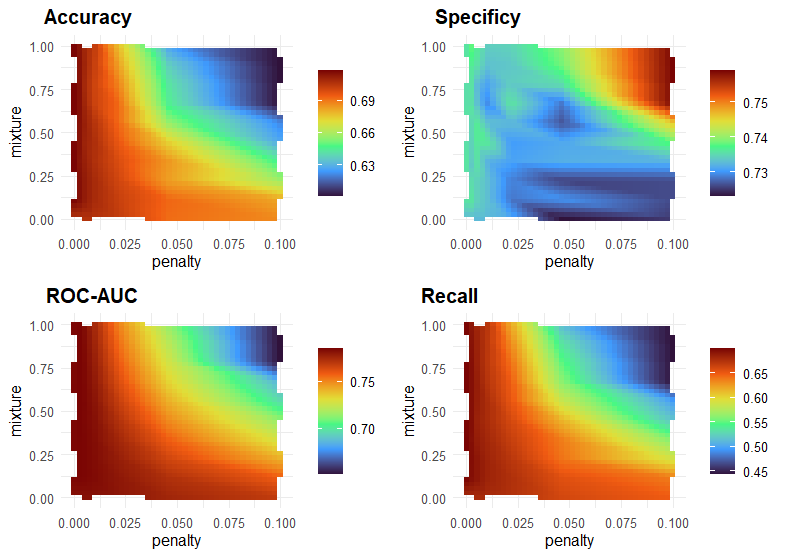
\includegraphics[width =0.7\textwidth]{graficos/lr_tuningplot.png}
\caption[Métricas de rendimiento de los modelos de Regresión Logística con penalización]{Métricas de rendimiento de los modelos de Regresión Logística con penalización.  \it Fuente: Elaboración propia.}
\label{fig:lr_tuningplot}
\end{figure}

Finalmente, se elige el modelo maximiza la tasa de acierto, cuyos
parámetros son: \(\alpha= 1\) y \(\lambda = 0.000464\). Es decir, un
modelo de Regresión Logística \emph{lasso} puro. Los coeficientes de
este modelo se muestran en la Figura \ref{fig:lr_coef} del {[}Apéndice
A.2. Salidas de los modelos{]}{[}Salidas de los modelos{]}.

\hypertarget{regresiuxf3n-loguxedstica-con-penalizaciuxf3n-usando-pca}{%
\section{Regresión Logística con penalización usando
PCA}\label{regresiuxf3n-loguxedstica-con-penalizaciuxf3n-usando-pca}}

A continuación se considera el mismo modelo de Regresión Logística con
penalización que en la sección, anterior pero en lugar de trabajar con
los datos directamente, se aplica análisis de componentes principales
sobre los datos normalizados en el preprocesamiento, ajustando el número
de componentes principales utilizadas. Para construir el \emph{grid} de
parámetros se consideran los mismos valores que en el modelo sin PCA
para los parámetros de penalización y mezcla pero ahora se consideran
también 7 posibles valores para el número de componentes principales
(\(\{20,25,30,...,50\}\)). Nótese que anteriormente, cuando se realizó
PCA en la {[}Sección 4.3{]}{[}Análisis multivariantes de las variables
numéricas{]} tan solo se consideraron las 18 variables numéricas del
conjunto de datos antes de aplicar ingeniería de características, y se
concluyó que eran necesarias al menos 14 componentes principales para
explicar el 90\% de la varianza de los datos. En cambio, aquí se están
considerando todas las variables después de aplicar ingeniería de
características, por lo que se están incluyendo todas las variables
\emph{dummy} creadas a partir de los factores. Esto supone un total de
59 variables (véase la Figura \ref{fig:lr_coef} del {[}Apéndice
A.2{]}{[}Salidas de los modelos{]}, donde aparecen todas las variables
del modelo una vez aplicada ingeniería de características), por lo que
es de esperar que el número de componentes principales necesarias para
explicar un porcentaje alto de la varianza de los datos aumente
sensiblemente con respecto a los resultados obtenidos considerando tan
solo las variables numéricas. Es por ello que se consideran al menos 20
componentes principales en el ajuste.

Finalmente, el modelo que maximiza la tasa de acierto es el que tiene 40
componentes principales, \(\alpha= 0.333\) y \(\lambda = 0.00464\).

\hypertarget{uxe1rboles-de-decisiuxf3n}{%
\section{Árboles de Decisión}\label{uxe1rboles-de-decisiuxf3n}}

Se construirán los Árboles de Decisión usando el índice de Gini como
medida de impureza utilizada para determinar el par variable-corte en
cada nodo, y se elegirá el parámetro de coste-complejidad (\(\alpha\))
que maximice la tasa de acierto. Tras valorar también el uso de la
Entropía como medida de impureza y realizar algunas pruebas previas,
finalmente se optó por usar el índice de Gini, ya que viene implementado
en los paquetes considerados y que, en las pruebas realizadas, el uso de
una medida u otra no supuso cambios significativos en los resultados
obtenidos. Se considera un \emph{grid} con 10 valores del parámetro de
coste-complejidad que oscilan entre \(1.28e-10\) y \(3.02e- 2\). La
mejor tasa de acierto en el conjunto de validación se obtiene con
\(\alpha = 0.00182\). En la Figura \ref{fig:dt_tuningplot} se muestran
las distintas métricas de rendimiento sobre los datos de validación para
cada uno de los valores del parámetro a ajustar.

\begin{figure}[h!]
\centering
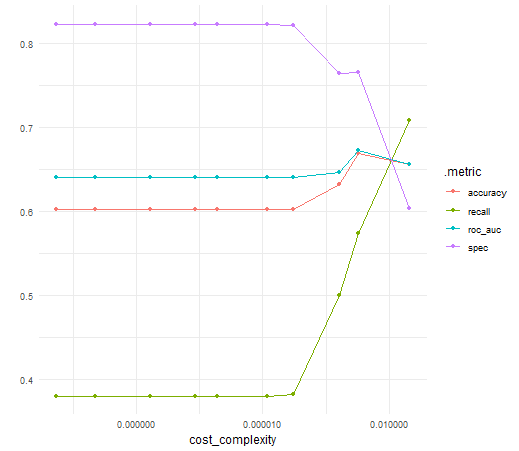
\includegraphics[width =0.7\textwidth]{graficos/dt_tuningplot.png}
\caption[Métricas de rendimiento del Árbol de Decisión en función de $\alpha$]{Métricas de rendimiento del Árbol de Decisión en función del parámetro de coste-complejidad. \it Fuente: Elaboración propia.}
\label{fig:dt_tuningplot}
\end{figure}

\hypertarget{bosques-aleatorios}{%
\section{Bosques Aleatorios}\label{bosques-aleatorios}}

En este modelo se han ajustado los parámetros \emph{mtry} (el número de
variables que se seleccionarán aleatoriamente en cada nodo) y
\emph{min\_n} (el número de observaciones en un nodo a partir del cual
no se sigue dividiendo y se convierte en nodo hoja). En este caso se ha
optado por un enfoque diferente, motivado por el amplio rango de valores
que puede tomar el parámetro \emph{min\_n} y por las limitaciones
computacionales del equipo disponible. Tras realizar varias pruebas se
ha observado que, con estos datos, al ajustar el parámetro \emph{trees}
(el número de árboles a considerar) no se obtiene una mejorar
significativa de los resultados frente a considerar el valor por defecto
de 1000 árboles, por lo que se ha preferido dejar este parámetro fijo.

De esta forma, la estimación de parámetros se ha hecho en dos etapas. En
una primera etapa se ha fijado el parámetro \(mtry = 4\) y se ha
estimado el parámetro \emph{min\_n} considerando para ello un
\emph{grid} equiespaciado de 1000 a 2500 tomando valores de 100 en 100
(\(\{1000,1100,...,2500\}\)). Para elegir entre los distintos modelos,
esta vez se ha usado como criterio la sensibilidad, obteniendo el valor
más elevado para \(min\_n = 2100\). En la segunda etapa, una vez
\emph{min\_n}, este se ha considerado fijo y se ha estimado \emph{mtry},
considerando una rejilla de 10 valores equiespaciados tomados del 1 al
10 (\(\{1,2,...,10\}\)). De nuevo se ha utilizado la sensibilidad para
elegir el modelo final, eligiendo así \(min\_n = 7\). En la Figura
\ref{fig:rf_tuningplot} se recogen los resultados de las dos etapas de
\emph{tuning}. El modelo final elegido tiene \(min\_n = 2100\) y
\(mtry = 7\).

Aquí es necesario hacer un inciso sobre el motivo de considerar valores
de \(min\_n\) tan elevados, en especial si se tiene en cuenta que la
muestra con la que se trabaja está formada por 20.000 registros. En un
inicio, se trató de ajustar ambos parámetros a la vez, considerando
valores usuales para el parámetro \(min_n\) (del orden de la decena).
Sin embargo, los tiempos de entrenamiento eran sumamente largos y el
rendimiento de los modelos era pésimo. Si bien el área bajo la curva ROC
y la tasa global de acierto eran aceptables y la tasa de acierto en la
clase negativa era excelente, en la clase positiva las tasas de acierto
obtenidas era inferiores a 0.5, indicando que los modelos no estaban
funcionando adecuadamente. Entonces, se comenzaron a realizar pruebas
con valores más elevados de \(min\_n\), hasta conseguir un rendimiento
aceptable en la clase positiva, que es lo principal en este problema. De
esta forma, se llegó a los valores del parámetro \(min\_n\) que se
presentan en el párrafo anterior, que llevan a considerar árboles poco
profundos. Sería interesante, en trabajos futuros, seguir explorando
vías de mejora de este modelo, tratando de desentrañar las causas del
rendimiento poco prometedor obtenido con valores de \(min\_n\)
moderados.

\begin{figure}[h!]
\centering
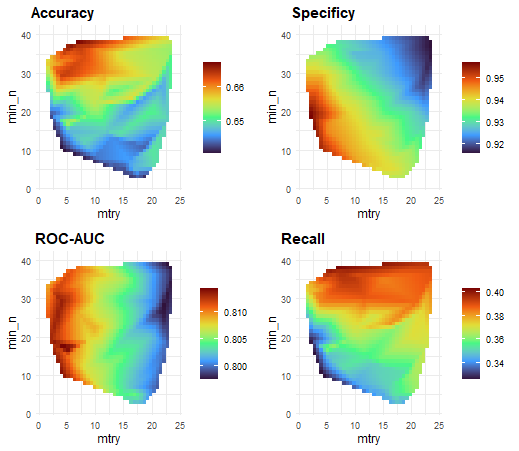
\includegraphics[width =\textwidth]{graficos/rf_tuningplot.png}
\caption[Métricas de rendimiento de \textit{Random Forest} en función de los parámetros]{Métricas de rendimiento de \textit{Random Forest} en función de los parámetros.  \it Fuente: Elaboración propia.}
\label{fig:rf_tuningplot}
\end{figure}

\hypertarget{knn}{%
\section{KNN}\label{knn}}

Para aplicar el modelo, primero se han transformado las variables
categóricas en variables \emph{dummy} y, posteriormente, se han
tipificado todas las variables. Se ha usado la distancia euclídea entre
los vectores transformados. Para ajustar el parámetro \(k\) del modelo
se han tomado valores entre 1 y 400. La mayor tasa de acierto sobre los
datos de validación se ha obtenido con \(k = 275\). Los resultados del
\emph{tuning} se muestran en la Figura \ref{fig:knn_tuningplot}.

\begin{figure}[h!]
\centering
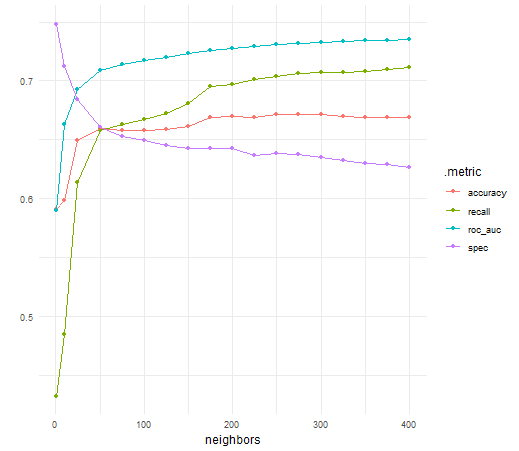
\includegraphics[width =0.7\textwidth]{graficos/knn_tuningplot.png}
\caption[Métricas de rendimiento de KNN en función de $k$]{Métricas de rendimiento de KNN en función del número de vecinos. \it Fuente: Elaboración propia.}
\label{fig:knn_tuningplot}
\end{figure}

\hypertarget{svm-lineal}{%
\section{SVM lineal}\label{svm-lineal}}

Antes de construir el modelo, se han transformado las variables
categóricas usando variables \emph{dummy} y se han tipificado todas las
variables. Se ha probado con 15 valores del parámetro \emph{coste} entre
0.001949 y 24.666648. La mayor tasa de acierto y el mayor \emph{recall}
se han obtenido para \(C = 0.0437\). Los resultados del \emph{tuning} se
muestran en la Figura \ref{fig:svm_tuningplot}.

\begin{figure}[h!]
\centering
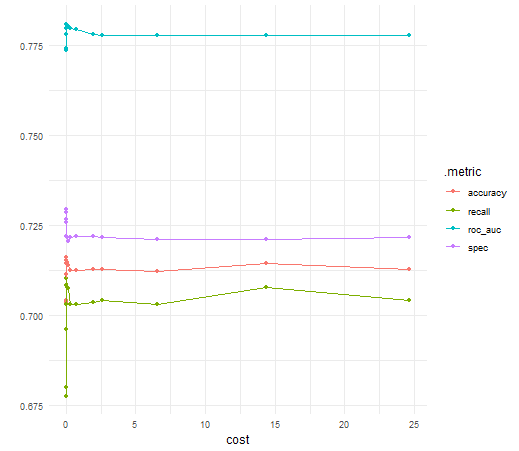
\includegraphics[width =0.7\textwidth]{graficos/svm_tuningplot.png}
\caption[Métricas de rendimiento de SVM en función del parámetro $coste$]{Métricas de rendimiento de SVM en función del parámetro $C$. \it Fuente: Elaboración propia.}
\label{fig:svm_tuningplot}
\end{figure}

\hypertarget{svm-radial}{%
\section{SVM radial}\label{svm-radial}}

Por último, se ha construido el modelo de SVM usando un \emph{kernel}
gaussiano, con la intención de comprobar si el uso de esta función
kernel es capaz de mejorar la separabilidad de los datos. Se ha
considerado este \emph{kernel} y no otro por ser el de uso más común. El
preprocesamiento ha sido el mismo que en el caso del \emph{kernel}
lineal. Dado el elevado tiempo de entrenamiento de este modelo solo se
ha probado con 8 combinaciones de valores para los parámetros \(C\) y
\(\gamma\), que oscilan entre 0.005 y 31.7 y entre 0 y 0.05,
respectivamente. La mayor tasa de acierto sobre los datos de validación
se ha conseguido para \(C = 31.7\) y \(\gamma = 0.0000496\).

\hypertarget{evaluaciuxf3n-y-comparaciuxf3n-de-modelos}{%
\section{Evaluación y comparación de
modelos}\label{evaluaciuxf3n-y-comparaciuxf3n-de-modelos}}

\hypertarget{comparativa-sobre-el-conjunto-de-validaciuxf3n}{%
\subsection{Comparativa sobre el conjunto de
validación}\label{comparativa-sobre-el-conjunto-de-validaciuxf3n}}

A continuación se muestran las métricas de cada uno de los modelos
seleccionados en los datos de validación en la Tabla
\ref{tab:metricas_val} y en la Figura \ref{fig:validation_metrics}. Las
curvas ROC de todos los modelos se muestran en la Figura
\ref{fig:roc_validation}.

Puede observarse que los resultados obtenidos por todos los modelos son
bastante similares. Destacan el modelo de Bosque Aleatorio y el de
Regresión Logística con penalización, el primero por ser el que tiene la
tasa de acierto y la sensibilidad más elevadas, y el segundo por dar los
mejores resultado en cuanto a precisión y especificidad. Las curvas ROC
de los modelos de bosque aleatorio, regresión logística con
penalización, SVM lineal y SVM radial son prácticamente iguales. Los
modelos más pobres son la regresión logística aplicando PCA, KNN y el
árbol de decisión. Seguramente, esto sea debido a que son modelos
demasiado simples dada la complejidad del problema al que se quieren
aplicar.

\begin{table}[H]
\centering
\resizebox{0.5\columnwidth}{!}{%
\begin{tabular}{@{}llllll@{}}
\toprule
model\_name & roc\_auc & accuracy & recall & specificity & precision \\ \midrule
lr          & 0.785    & 0.719    & 0.700  & 0.738       & 0.727     \\
lr\_pca     & 0.727    & 0.659    & 0.624  & 0.694       & 0.670     \\
dt          & 0.656    & 0.656    & 0.709  & 0.604       & 0.641     \\
rf          & 0.781    & 0.725    & 0.758  & 0.693       & 0.711     \\
svm\_linear & 0.781    & 0.716    & 0.710  & 0.722       & 0.718     \\
svm\_rbf    & 0.777    & 0.710    & 0.692  & 0.728       & 0.717     \\
knn         & 0.732    & 0.672    & 0.706  & 0.637       & 0.660     \\ \bottomrule
\end{tabular}%
}
\caption[Métricas de los modelos seleccionados sobre el conjunto de validación]{Métricas de los modelos seleccionados sobre el conjunto de validación.  \it Fuente: Elaboración propia.}
\label{tab:metricas_val}
\end{table}

\begin{figure}[H]
\centering
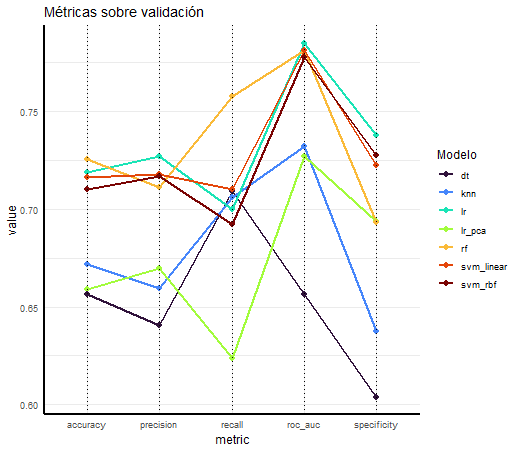
\includegraphics[width =0.7\textwidth]{graficos/validation_metrics.png}
\caption[Gráfico de métricas obtenidas sobre el conjunto de validación]{Gráfico de métricas obtenidas sobre el conjunto de validación por cada uno de los modelos seleccionados. \it Fuente: Elaboración propia.}
\label{fig:validation_metrics}
\end{figure}

\begin{figure}[H]
\centering
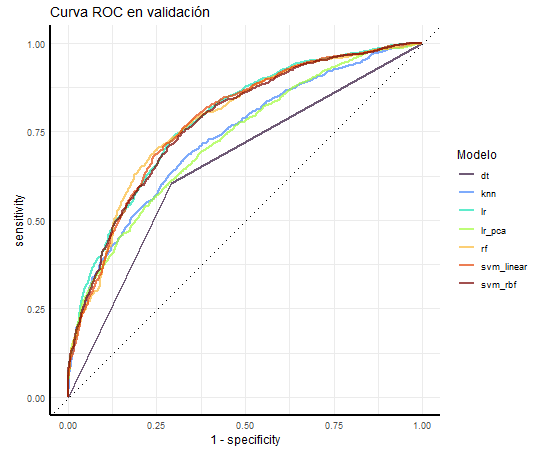
\includegraphics[width =0.7\textwidth]{graficos/roc_validation.png}
\caption[Curvas ROC sobre el conjunto de validación]{Curvas ROC sobre el conjunto de validación. \it Fuente: Elaboración propia.}
\label{fig:roc_validation}
\end{figure}

A continuación, se incluye un fragmento del código en el que se ilustra
el uso de funciones propias del flujo de trabajo habitual de
\emph{tidymodels} dentro de la filosofía \emph{``tidy data''} propia del
ecosistema \emph{tidyverse}, haciendo uso de estructuras anidadas y
funciones de orden superior. En este fragmento, se selecciona la mejor
combinación de parámetros para cada modelo, usando la tasa de acierto
global como criterio; a continuación, se obtienen todas las medidas de
rendimiento sobre el conjunto de validación para cada modelo ajustado,
haciendo uso de la función propia \texttt{get\_metrics}; y por último,
se crea la curva ROC de cada modelo ajustado sobre el conjunto de
validación. El objeto \texttt{models\_tune} contiene los resultados del
ajuste de cada combinación de parámetros considerada para cada modelo
sobre el conjunto de validación.

\begin{Shaded}
\begin{Highlighting}[]
\NormalTok{models }\OtherTok{=}\NormalTok{ models }\SpecialCharTok{\%\textgreater{}\%} 
  \FunctionTok{mutate}\NormalTok{(}\AttributeTok{best\_tuning =} \FunctionTok{map}\NormalTok{(models\_tune, }
                           \ControlFlowTok{function}\NormalTok{(x) }\FunctionTok{select\_best}\NormalTok{(x, }
                                                   \AttributeTok{metric =} \StringTok{"accuracy"}\NormalTok{)),}
         \AttributeTok{best\_metrics =} \FunctionTok{map2}\NormalTok{(models\_tune,}
\NormalTok{                             best\_tuning,       }
                             \SpecialCharTok{\textasciitilde{}} \FunctionTok{collect\_predictions}\NormalTok{(.x,}
                                                   \AttributeTok{parameters =}\NormalTok{ .y) }\SpecialCharTok{\%\textgreater{}\%}    
                               \FunctionTok{get\_metrics}\NormalTok{() }\SpecialCharTok{\%\textgreater{}\%}          
                               \FunctionTok{extract2}\NormalTok{(}\DecValTok{1}\NormalTok{)), }
         \AttributeTok{roc =} \FunctionTok{map2}\NormalTok{(models\_tune,}
\NormalTok{                    best\_tuning,}
                    \SpecialCharTok{\textasciitilde{}} \FunctionTok{collect\_predictions}\NormalTok{(.x,}
                                          \AttributeTok{parameters =}\NormalTok{ .y) }\SpecialCharTok{\%\textgreater{}\%}    
                      \FunctionTok{roc\_curve}\NormalTok{(fire, .pred\_0))}
\NormalTok{         ) }
\end{Highlighting}
\end{Shaded}

\hypertarget{comparativa-sobre-el-cojunto-test}{%
\section{Comparativa sobre el cojunto
test}\label{comparativa-sobre-el-cojunto-test}}

Por último, para conocer la capacidad de generalización de los modelos
construidos, estos se evaluarán sobre nuevas observaciones, el conjunto
de datos test. Recuérdese que el entrenamiento de los modelos se ha
realizado con el conjunto de entrenamiento, formado por 12.927
observaciones tomadas entre el 2002 y mediados de 2014, y para ajustar
los parámetros de cada modelo, se han utilizado 4.309 observaciones
tomadas entre mediados de 2014 y mediados de 2019. Finalmente, se
evaluará la capacidad de predicción de los modelos sobre 4.310 nuevas
observaciones tomadas entre mediados de 2019 y 2022. Para ello, primero
se unirán los conjuntos de entrenamiento y validación para reentrenar
los modelos con la configuración de parámetros seleccionada en cada
caso, y posteriormente se compararán los valores predichos por los
modelos con los valores reales. Los resultados obtenidos se muestran en
la Tabla \ref{tab:metricas_test} y el la Figura \ref{fig:test_metrics}.
Las curvas ROC de los distintos modelos sobre el conjunto de datos test
se muestra en la Figura \ref{fig:roc_test}.

En este caso, los mejores resultados en todas las medidas los da el
modelo de Regresión Logística con penalización. Los modelos de SVM
muestran resultados bastante similares entre ellos y prácticamente
iguales al modelo de Regresión Logística. Sobre los datos test, el
modelo de Bosque Aleatorio ha dado un rendimiento peor que el obtenido
en validación, quedando por detrás de los tres modelos ya comentados,
aunque la sensibilidad de todos estos modelos es prácticamente igual. De
nuevo, los peores resultados los dan los modelos de Regresión Logística
aplicando PCA y el Árbol de Decisión, seguidos del KNN.

\begin{table}[H]
\centering
\resizebox{0.5\columnwidth}{!}{%
\begin{tabular}{@{}llllll@{}}
\toprule
model\_name & roc\_auc & accuracy & recall & specificity & precision \\ \midrule
lr          & 0.795    & 0.710    & 0.726  & 0.693       & 0.718     \\
lr\_pca     & 0.715    & 0.645    & 0.631  & 0.661       & 0.667     \\
dt          & 0.667    & 0.668    & 0.712  & 0.621       & 0.670     \\
rf          & 0.762    & 0.699    & 0.727  & 0.669       & 0.703     \\
svm\_linear & 0.790    & 0.705    & 0.729  & 0.680       & 0.710     \\
svm\_rbf    & 0.789    & 0.706    & 0.727  & 0.683       & 0.712     \\
knn         & 0.744    & 0.673    & 0.719  & 0.624       & 0.673     \\ \bottomrule
\end{tabular}%
}
\caption[Métricas sobre el conjunto test]{Métricas sobre el conjunto test. \it Fuente: Elaboración propia.}
\label{tab:metricas_test}
\end{table}

\begin{figure}[H]
\centering
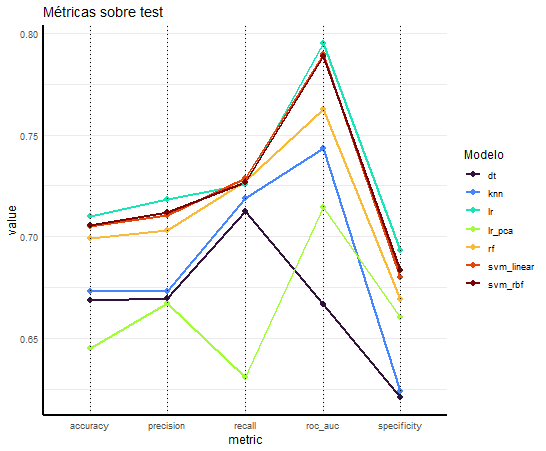
\includegraphics[width =0.7\textwidth]{graficos/test_metrics.png}
\caption[Gráfico de métricas obtenidas sobre el conjunto test]{Métricas obtenidas sobre el conjunto test por cada uno de los modelos seleccionados. \it Fuente: Elaboración propia.}
\label{fig:test_metrics}
\end{figure}

\begin{figure}[H]
\centering
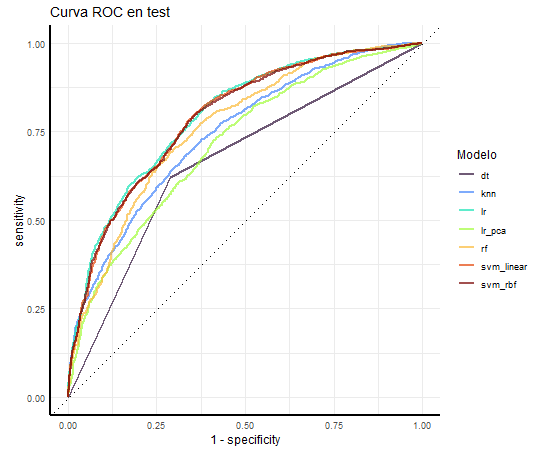
\includegraphics[width =0.7\textwidth]{graficos/roc_test.png}
\caption[Curvas ROC sobre test]{Curvas ROC sobre test. \it Fuente: Elaboración propia.}
\label{fig:roc_test}
\end{figure}

En el fragmento de código que se incluye a continuación, se realizan las
siguientes operaciones sobre todos los modelos considerados:

\begin{enumerate}
\def\labelenumi{\arabic{enumi}.}
\tightlist
\item
  Se finaliza el entrenamiento de los modelos, usando la combinación de
  parámetros previamente seleccionada para cada uno.
\item
  Se reentrenan sobre la unión de los conjuntos de entrenamiento y
  validación.
\item
  Se obtienen las medidas de rendimiento sobre el conjunto test.
\item
  Se construye la curva ROC de cada modelo sobre el conjunto test
\end{enumerate}

\begin{Shaded}
\begin{Highlighting}[]
\NormalTok{models }\OtherTok{=}\NormalTok{ models }\SpecialCharTok{\%\textgreater{}\%} 
  \FunctionTok{mutate}\NormalTok{(}\AttributeTok{final\_workflow =} \FunctionTok{map2}\NormalTok{(models\_workflow, }
\NormalTok{                               best\_tuning, }
\NormalTok{                               finalize\_workflow),}
         \AttributeTok{last\_fit =} \FunctionTok{map}\NormalTok{(final\_workflow, }
                        \ControlFlowTok{function}\NormalTok{(x) }\FunctionTok{last\_fit}\NormalTok{(x,}
\NormalTok{                                             splits,}
                                             \AttributeTok{add\_validation\_set=}\NormalTok{T)),}
         \AttributeTok{test\_metrics =} \FunctionTok{map}\NormalTok{(last\_fit,      }
                            \SpecialCharTok{\textasciitilde{}}\FunctionTok{collect\_predictions}\NormalTok{(.x) }\SpecialCharTok{\%\textgreater{}\%}  
                              \FunctionTok{get\_metrics}\NormalTok{() }\SpecialCharTok{\%\textgreater{}\%}  
                              \FunctionTok{extract2}\NormalTok{(}\DecValTok{1}\NormalTok{)), }
         \AttributeTok{test\_roc =} \FunctionTok{map}\NormalTok{(last\_fit,}
                        \SpecialCharTok{\textasciitilde{}}\FunctionTok{collect\_predictions}\NormalTok{(.x) }\SpecialCharTok{\%\textgreater{}\%}     
                          \FunctionTok{roc\_curve}\NormalTok{(fire, .pred\_0)) }
\NormalTok{         )}
\end{Highlighting}
\end{Shaded}

La fácil compresión del código, la posibilidad de usar funciones de
orden superior que permiten realizar operaciones a múltiples elementos
de forma sencilla y eficiente, y el uso de estructuras anidadas y
funciones de orden superior que simplifican la programación, muestran la
potencia de la integración de \emph{tidymodels} dentro del universo
\emph{tidyverse}.

En el siguiente capítulo, se evaluará el rendimiento de los modelos
construidos en esta sección al ser aplicados a dos casos prácticos. De
esta forma, se podrá valorar la utilidad de estos en la realidad y
conocer sus limitaciones.

\bibliography{bib/library.bib,bib/paquetes.bib}


%


\end{document}
